\chapter{Mechanizmy współbieżne Pythona}
W tym rozdziale chciałbym przedstawić mechanizmy, których programiści Pythona używaj, aby umożiwić pracę z językiem w trybie współbieżności. W celu zaprezentowania możliwości tych narzędzi stworzyłem prostą aplikację CLI\footnote{Command-line interface}, która korzysta z wszystkich przedstawionych w tym rozdziale rozwiązań.

\section{Opis narzędzia}
Narzędzie, które stworzyłem do zaprezentowania możliwości współbieżnych mechanizmów Pythona to proste CLI. Uruchamiamy je poleceniem:
\begin{lstlisting}
python main.py
\end{lstlisting}
, jednak w przedstawionej postaci nie będzie ono działało poprawnie, gdyż wymagane jest podanie co najmniej dwóch argumentów. Dwa obowiązkowe argumenty to po pierwsze czy chcemy korzystać z prostej implementacji czy implementacji wykonanej przy pomocy modułu concurrent.futures. Drugi argument wyznacza czy chcemy korzystać z modułu threading czy multiprocessing. Oddzielnym trybem jest krozystanie asyncio, w którym to przypadku w oba miejsca podajemy słowo asyncio.

Przydatnym argumentem będzie flaga -io, która gdy dodana będzie zmuszała nasz program do wykonania operacji wejścia-wyjścia - bez tego argumentu program domyślnie będzie wykonywał operacje związane z procesorem.

Dodatkowymi argumentami z których możemy skorzystać jest argument -visuals, który pozwoli nam obejrzeć przebieg działań na wykresach oraz -real-time, który włączy tryb dzięki któremu będziemy mogli dokładniej prześledzić przeplot działań naszego programu. Do wygenerowania wykresów użyta została biblioteka matplotlib\footnote{\url{https://matplotlib.org/}}.

Przykładowo jeśli chcemy zobaczyć jak będzie zachowywał się multiprocessing dla operacji wejścia wyjścia i ile każdy proces zajmie czasu podejamy polecenie:
\begin{lstlisting}
python main.py pool processing -io -visuals
\end{lstlisting}

\subsection{potencjalne operacje}
Przykładowymi operacjami zaimplementowanymi do mojego programu są: wykonywanie zapytań http oraz wykonywanie obliczeń. Funkcje odpowiedzialne za te procesy można znaleź w plikach o nazwach odpowiednio ,,downloading\_pages.py'' oraz ,,cpu\_heavy.py'', znajdujących się w katalogu ,,utils''.

\section{threading i multiprocessing}
Pierwszym mechanizmem, którym zajmiemy się w tym rozdziale jest moduł threading. Jest to moduł, który udostępnia nam interfejs do korzystania z niżej poziomowego modułu ,,\_thread''. Teoretycznie moduł ten umożliwia nam pracę z wieloma wątkami, jednak we wersji Pythona, o której piszę\footnote{CPython} ze względu na obecność Global Interpreter Lock wciąż kod będzie wykonywany przez tylko jeden wątek, który będzie przełączał się między zadaniami.\footnote{\url{https://docs.python.org/3/library/threading.html}}
\subsection{implementacja prosta}
Zaczniemy od wyjaśnienia sposobu implementacji tylko za pomocą modułu threading, bez korzystania z pomocniczych bibliotek języka. Funkcja, która będzie odpowiedzialna za włączanie kolejnych wątków wygląda następująco:
\begin{lstlisting}
from threading import Thread
from typing import Callable

def simple_threading(function_to_be_triggered: Callable, length=10) -> None:
    threads = []
    for i in range(length):
        threads.append(Thread(target=function_to_be_triggered, args=(i,)))
    for thread in threads:
        thread.start()
    for thread in threads:
        thread.join()
\end{lstlisting}
Jako argumenty funkcji podana jest najpierw funkcja, która ma być wykonywana, a następnie konkretna ilość wykonań podanej funkcji.Do listy wątków najpierw dodajemy instancje klasy Thread, w następnej kolejności po kolei startujemy każdy z wątków, a na koniec dołączamy każdy wątek do wykonania programu, aby program zaczekał na zakończenie wszystkich dołączonych wątków.

W wypadku multiprocessingu implementacja rozwiązania prostego wygląda tak samo, zmianie ulega jedynie zaimportowana klasa Thread. Zamiast niej importujemy klasę Process:
\begin{lstlisting}
from multiprocessing import Process
\end{lstlisting}
i używamy jej w tym samym miejscu co klasę Thread. Sposób zapisuej pozostaje ten sam, lecz zmienai się zasada działania programu, który przy każdym użyciu metody start() na instancji Processu włącza nowy interpreter Pythona i wykonuje w nim zadany kod.

\subsection{Implementacja za pomocą Executora}
Implementacja za pomocą Executora jest implementacją mniej skomplikowaną używającą modułu concurrent.futures, który powstał właśnie w celu usprawnienia pracy z modułami threading i multiprocessing poprzez dostarczenie wysokopoziomowego interfejsu dla tych narzędzi.
Funkcja odpowiedzialna za planowanie wykonań wygląda następująco:
\begin{lstlisting}
from concurrent.futures import ThreadPoolExecutor
from typing import Callable


def pool_processing(function_to_be_triggered: Callable, length=10) -> list:
    with ThreadPoolExecutor() as ex:
        res = ex.map(function_to_be_triggered, range(length))
    return list(res)
\end{lstlisting}
W tym przypadku argumenty podawane do funkcji pozstają dokładnie takie same jak w przypadku implementacji prostej. Za pomocą context managera tworzymy instancję ThreadPoolExecutora i następnie korzystamy z jego metody map, która automatycznie pobiera wszystkie elementy generatora podanego jako drugi argument i przekazuje je pojedynczo do wybranej funkcji podanej jako pierwszy argument. Dla każdego elementu tego generatora zostaje użyty kolejny wątek.

Ponownie implementacja rozwiązania korzystającego z multiprocessingu jest prawie identyczna i różni się jedynie użytą klasą Executora, która tym razem zaimportowana jest następująco:
\begin{lstlisting}
from concurrent.futures import ProcessPoolExecutor
\end{lstlisting}

\section{asyncio}
Rozwiązanie za pomocą asyncio różni się znacząco wobec poprzednich solucji. 

\newpage
\section{Wykresy}
Tutaj możemy przyjrzeć się kilku wynikom czasowym różnych operacji wyknywanych za pomocą innego mechanizmu współbieżnego.
\begin{figure}[h]
    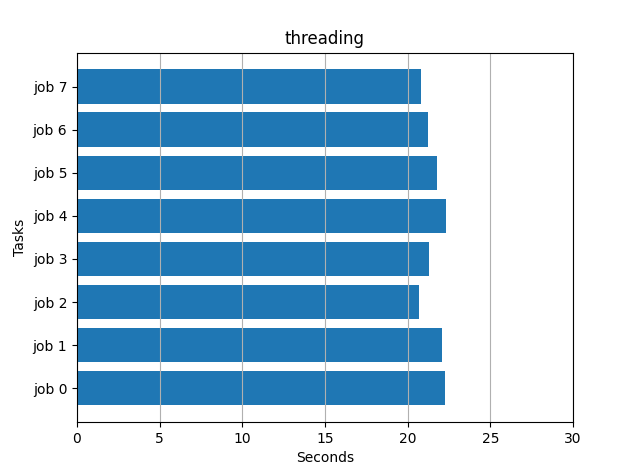
\includegraphics{zdjecia/threading_requests}
    \caption{Czasy działania threadingu przy operacji wysyłania zapytań http}
\end{figure}

\begin{figure}
    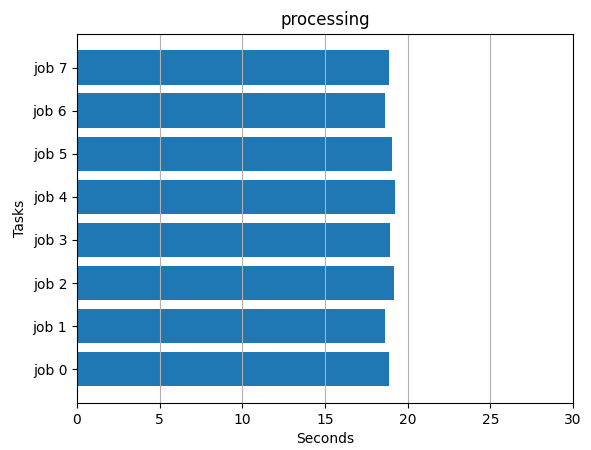
\includegraphics{zdjecia/processing_requests}
    \caption{Czasy działania multiprocessingu przy operacji wysyłania zapytań http}
\end{figure}

\begin{figure}
    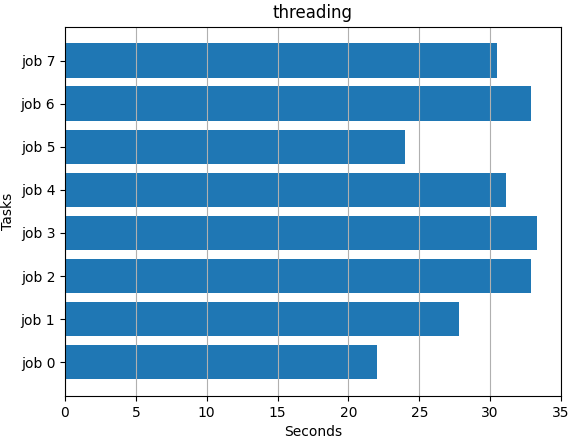
\includegraphics{zdjecia/threading_cpu}
    \caption{Czasy działania threadingu przy operacji związanej z procesorem}
\end{figure}

\begin{figure}
    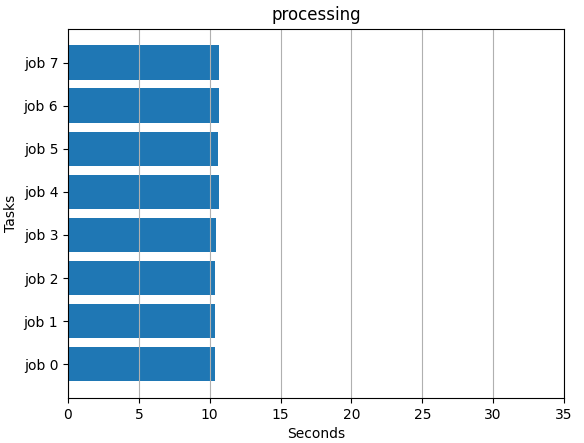
\includegraphics{zdjecia/processing_cpu}
    \caption{Czasy działania multiprocessingu przy operacji zwiżanej z procesorem}
\end{figure}
